\documentclass[]{final_report}
\usepackage{graphicx}
\usepackage{hyperref}
\usepackage[final]{pdfpages}
\usepackage{booktabs}
\usepackage{multirow}
\usepackage{framed}
\usepackage{caption}
\usepackage{tikz}
\usetikzlibrary{timeline}
\usepackage{dirtree}

%%%%%%%%%%%%%%%%%%%%%%
%%% Input project details
\def\studentname{James King}
\def\reportyear{2018}
\def\projecttitle{Cooperative Strategies in Multi-Agent Systems}
\def\supervisorname{Kostas Stathis}
\def\degree{BSc (Hons) in Computer Science}
\def\fullOrHalfUnit{Full Unit} % indicate if you are doing the project as a Full Unit or Half Unit
\def\finalOrInterim{Final Report} % indicate if this document is your Final Report or Interim Report

\begin{document}

Tips:
\begin{itemize}
	\item Communicate with Kostas
	\item Use figures!
	\item Ensure structure is flowing
	\item Use sources for everything
\end{itemize}
To Do:
\begin{itemize}
	\item Describe appendix
	\item Act on Interim Review Feedback
	\item Act on planning and timescale comments from interim report
	\item Act on contents of summary of completed work from interim report
	\item Change the Rationale to fit Final report
	\item Write a literature review or combine with Rationale and add to it?
	\item Write Contents and Knowledge
	\item Write critical analysis and discussion
	\item Write professional issues (get background reading and citations)
\end{itemize}
	
\maketitle

%%%%%%%%%%%%%%%%%%%%%%
%%% Declaration

\chapter*{Declaration}

This report has been prepared on the basis of my own work. Where other published and unpublished source materials have been used, these have been acknowledged.

\vskip3em

Word Count:

\vskip3em

Student Name: \studentname

\vskip3em

Date of Submission: \today

\vskip3em

Signature: \\

\includegraphics[scale=0.05]{Signature.png}

\newpage

%%%%%%%%%%%%%%%%%%%%%%
%%% Table of Contents
\tableofcontents\pdfbookmark[0]{Table of Contents}{toc}\newpage

%%%%%%%%%%%%%%%%%%%%%%
%%% Your Abstract here

\begin{abstract}
Intelligent agents and multi-agent systems are burgeoning technologies with the potential to impact society on a huge scale. There is a key talking point in the development of multi-agent systems about how to encourage cooperation between agents. Agents act autonomously and as such their internal state and intentions remain unknown to other agents.\\
This is similar to an early issue in the theory of evolution. The issue being; how does cooperation evolve in a world where natural selection pushes towards competition? A number of solutions have been proposed historically, including game-theoretic mechanisms to aid the evolution of cooperation.\\
There is a juncture here between the study of evolutionary theory and multi-agent systems. Marrying the areas of study could be the key to opening up a world of possibilities in which agents cooperate and provide solutions to big problems. But how can we develop systems that achieve this? What mechanisms can we use in developing these systems?\\
In my project I have been and will continue to be exploring these questions. My method for exploring these questions is reviewing past work and then developing a model to put them to a practical test, and then analysing the outcome of these practical tests.
\end{abstract}
\newpage

\chapter{Rationale}
\section{The Problem}
\label{section:problem}
To understand the aims and objectives of this project we must first grasp the history of the study of interaction between biological and computational agents (often known as intelligent agents in the field of computer science). It is important to distinguish between biological and computational agents as the study of natural selection and the evolution of cooperation in biological agents has a long and separate history from the study of intelligent agents in computer science.\\
The background to my project is covered in my first two reports (included in the appendix in chapter~\ref{appendix}). I will be applying this knowledge in a more convenient format for the interim report here, my two reports provide a more in depth study on the topic of the evolution of cooperation and indirect reciprocity.\\
As explained in my first report (on the evolution of cooperation in relation to game-theory and different game-theoretic mechanisms to aid it), early Darwinian evolutionary theory was groundbreaking, however both opponents and even proponents of evolution such as Peter Kropotkin~\cite{kropotkin1902mutual} (a Russian evolutionary scientist and political activist) found it fell short in explaining cooperative phenomena.\\
Cooperation is the idea of helping others at a detriment or cost to yourself. Of course, this concept is a key part of the natural world. For example, the act of parents supporting their children and vice-versa in human family groups. There are even interspecies examples such as that of the Meerkat and Drongo Bird~\cite{bbcafrica}.\\
The problematic question posed by the phenomena of cooperation is the idea from the theory evolution: the survival of the fittest~\cite{spencer1864principles}. This idea pushes individuals to compete for resources, so why does cooperation exist when there is a process actively pushing for competition? How did cooperation evolve in a world focused on competition?

\section{Cooperation Aids}
There have been a number of attempts to explain the phenomena of cooperation~\cite{kropotkin1902mutual, selfish_gene, evolution_of_cooperation, five_rules_coop}. In his book `The Selfish Gene'~\cite{selfish_gene} Richard Dawkins attempted to explain the idea that the real replicator in natural selection is the gene itself, which is self-interested in replication. As such, individuals are driven to working towards replication of the gene, not to improving our own personal fitness.\\
The idea of being driven towards the replication of our genes comes under the banner of Kinship Theory, highlighted by Axelrod and Hamilton in their paper~\cite{evolution_of_cooperation} as one of the theories seeking to explain cooperation. Hamilton wrote a paper on Kinship Theory earlier in his academic career~\cite{kinhamilton}, explaining his version in which agents are encouraged to cooperate as they are interested in improving `inclusive fitness' over their own individual fitness. Inclusive fitness refers to the fitness of both themselves and their relatives; the closer the relative the more they have an effect on an agent's inclusive fitness.\\
The main mechanism highlighted by Axelrod and Hamilton~\cite{evolution_of_cooperation} is, in popular culture, known as the game `the iterated prisoner's dilemma'. The iterated prisoner's dilemma uses the idea of direct reciprocity to aid in the evolution of cooperation. This idea being: if I scratch your back, you'll scratch  mine. In a round of the prisoner's dilemma, both agents simultaneously choose whether to cooperate or defect. A single prisoner's dilemma round provides no aid, but if the rounds are repeated, agents are encouraged to cooperate if historically there has been cooperation from the other agent with whom they're interacting. Another reason to cooperate is the payoff matrix given in table~\ref{tab:ipdpayoffmatrix}. Multiple rounds of both agents cooperating gives both higher social welfare (overall points accrued~\cite{kostas_deductive}) and greater individual payoff than multiple rounds of mutual defection.
\begin{framed}
	\begin{center}
		\begin{tabular}{c|c|c}
		\multirow{2}{*}{Player A} & \multicolumn{2}{c}{Player B}\\		
		& Cooperation & Defection\\
		\hline
		\multirow{2}{*}{Cooperation} & A=3 & A=0\\
		& B=3 & B=5\\
		\hline
		\multirow{2}{*}{Defection} & A=5 & A=1\\
		& B=0 & A=1\\
		\end{tabular}
		\captionof{table}{The payoff matrix in a typical iterated prisoner's dilemma game (such as Axelrod and Hamilton's). A=x, B=y where x denotes the payoff for A and y the payoff for B.}
		\label{tab:ipdpayoffmatrix}
	\end{center}	
\end{framed}
Direct reciprocity and Kinship Theory (or kin selection) are two of the five rules presented in Martin A. Nowak's paper `Five Rules for the Evolution of Cooperation'~\cite{five_rules_coop}. The other three rules use different versions of reciprocity mechanisms. Network reciprocity is similar to the iterated prisoner's dilemma. Axelrod and Hamilton's approach~\cite{evolution_of_cooperation} uses a round-robin tournament where all players interact with every other player. Network reciprocity is set aside from this style of direct reciprocity as it is played on a graph with players as the nodes, and the edges denoting who interacts with whom.\\
Another of the five rules, group selection, builds upon direct reciprocity. In group selection a population is separated out into smaller subpopulations. The players in these subpopulations only interact and reproduce within their subpopulation group. The group sizes fluctuate based on how fast agents reproduce inside them (dependent on the agents' fitness scores). If a group gets to a certain size, it has a chance of splitting, and when one group splits another group is removed. The effect of this is selection on two levels: individually and between groups, aiding the evolution of cooperation.\\
The last mechanism presented by Nowak and the one I am most interested in, is indirect reciprocity. The idea behind this mechanism is slightly less intuitive than direct reciprocity: if I scratch your back, hopefully later on someone else will remember and scratch my back. Actions in indirect reciprocity are different to direct reciprocity as they do not involve both agents acting. Only the donor of the donor-recipient interaction pair can choose to cooperate or defect, the payoffs of which are presented in table~\ref{tab:indirectpayoffmatrix}.
The indirect reciprocity mechanism utilizes the idea of reputation. Cooperative acts may result in bettering the donor's reputation whereas defecting may result in a loss of reputation. How agents view the reputation of another, depends upon their implementation. Two important implementations described in my second report are the standing strategy~\cite{leimarhammer} and using image scores~\cite{evol_indirect_image}. Agents have the opportunity to base their decisions on these reputations. Sommerfeld \textit{et al.}~\cite{gossip_alt} put forward that the social action of gossip can help agents spread information in regards to agents reputations.
\begin{framed}
	\begin{center}
		\begin{tabular}{c|c|c}
		\multirow{2}{*}{Donor Action} & \multicolumn{2}{c}{Payoffs}\\		
		& Donor & Recipient\\
		\hline
		Cooperation & -1 & 2\\
		\hline
		Defection & 0 & 0\\
		\end{tabular}
		\captionof{table}{The common payoff for most indirect reciprocity models}
		\label{tab:indirectpayoffmatrix}
	\end{center}	
\end{framed}

\section{Theory Surrounding Intelligent Agents and Multi-Agent Systems}
In my third report in the appendix chapter~\ref{appendix} I have covered the theory surrounding intelligent agents and multi-agent systems. Agents, as described by Russell and Norvig~\cite{russell2016artificial}, are anything that perceives and acts upon its environment. Agents can be built using a number of architectures, some of which are seemingly more intelligent than others. Russell and Norvig highlight 5 such architectures ranging from agents which simply act in reflex to their environment to agents that actively learn from their percepts.\\
The idea that an agent is anything the perceives and acts upon it's environment could be considered a `weak' notion of agency, even in comparison to Wooldridge and Jennings' `weak' notion of agency~\cite{wooldridge_jennings_1995}. Their paper stipulates that agents must be able to exhibit these 4 properties: autonomy, social ability, reactivity and proactivity.\\
Autonomy is considered to be operating without direct human or other agent intervention, with the agent having control over their internal state and actions. Social ability is defined as the ability of agents to interact with other agents (possibly biological) using an agent communication language. Reactivity is the ability to perceive their environment and act upon the changes in it. Proactivity makes Wooldridge and Jennings'~\cite{wooldridge_jennings_1995} notion stronger than Russell and Norvig's~\cite{russell2016artificial} as it stipulates agents must not simply be reactive to their environment but are also able to exhibit goal-directed behaviour.\\
To be able to satisfy the properties laid out by Wooldridge and Jennings~\cite{wooldridge_jennings_1995} and the definition of an agent from Russell and Norvig~\cite{russell2016artificial} agents need an environment to reside in. The possible environments are endless. An agent is built to work in a specific environment, the reason for an agents existence varies but often agents will attempt to complete specific tasks delegated to them.\\
Multi-agent systems are systems consisting of a combination of an environment and a number of agents perceiving and acting within it. Interactions can generally occur between both the environment and other agents in the system.


\section{Relevance of The Problem and Indirect Reciprocity to Multi-Agent Systems}
The societies which are simulated in the theories and experiments presented by Axelrod, Hamilton and Nowak~\cite{evolution_of_cooperation, five_rules_coop} are strikingly similar to multi-agent systems. The models include groups of players residing in an environment interacting with each other, leading naturally to using these game-theoretic approaches to modelling interactions in multi-agent systems.\\
As agents act autonomously in a multi-agent system, why should one agent cooperate with another at a cost to themselves? From a developer's viewpoint, they can see the possibilities that if agents work together agents can accomplish so many brilliant things. From the agent's viewpoint though, why should that agent trust that if they cooperate, their good actions will not be taken advantage of?\\
This is the problem in section~\ref{section:problem} reformulated for multi-agent systems. From a developer's perspective working on these sorts of systems, their goal is to encourage cooperation between agents but also not leave their agents or system of agents open to abuse. How can developers achieve this goal?\\
One way to approach this problem is to study how other environments have achieved this. One such environment that has achieved the evolution of cooperation, that we have identified earlier in this report, is the environment we live in, nature itself. Though nature encourages competition it has also led to cooperation between biological agents. So how can we learn from the processes nature employs?\\
We can apply the processes identified by game-theory and Kinship Theory to model multi-agent systems by implementing multi-agent systems that run these processes. Using a similar mechanism to indirect reciprocity Mui \textit{et al.}~\cite{Mui:2002:NRM:544741.544807} explored the role of reputation in the evolution of cooperation in multi-agent systems. The paper uses a number of different notions for reputation, one similar to Nowak's observer-based reputation, where an agent changes their view of another agent depending on the actions it views of the other agent. Their experiments found a large number of interactions were needed per generation for cooperative agents to dominate.\\
The mechanism/process I have chosen and outlined in my report on indirect reciprocity was chosen as I believe it applies well to multi-agent systems for a number of reasons. Firstly agents who interact across large networks such as the internet may never interact again, so it is imperative to have a strategy for deciding on how to act in these singular interactions. My models use of indirect reciprocity and reputation will allow us to study specifically these sort of `sparse' interactions and the effectiveness of strategies in these interactions.\\
Another reason I believe my model matches multi-agent systems well is the social ability that it comes with. Nowak and Sigmund highlighted the importance of knowing another agents reputation to the success of the evolution of cooperation in an indirect reciprocity system~\cite{evol_indirect_image}. They found that the probability of knowing another agents reputation had to be greater than the cost to benefit ratio of the action for cooperation to evolve.\\
In my system, agents who know each other will be able share information via gossip on other agents. The shared information increases the chances of knowing a certain agents reputation and in turn, helps defend against generally cooperative or `nice' agents from being exploited. However, it also leads to another avenue of attack through spreading misinformation. This mechanism of information sharing could be used as a defence against exploitation, but it is important to understand how best to implement it and how effective it is before such an option is chosen.\\
One of the four properties laid out by Wooldridge and Jennings~\cite{wooldridge_jennings_1995} is autonomy, which includes control over the agent's own internal state. The fact that in my model reputation is not a centrally managed concept but is part of the internal state, brings the system closer to a truly decentralised multi-agent system architecture.\\
Though reproduction itself doesn't, in fact, occur in multi-agent systems, it is likely that agent systems will be replaced and upgraded. The replacing systems will probably follow strategies that are known as effective by the developers. My reproduction mechanism aims to show how this replacement will take place, by assigning more likelihood for reproduction of an agent to occur if the strategy is successful. The reproduction may tend towards a defecting agent if they are more successful and vice-versa.\\
For further information on my model please refer to my second report on indirect reciprocity, strategies for agents and the development of a concrete model to implement in the appendix in chapter~\ref{appendix}.

\section{Project Specification, Aims and Objectives}
From the sections above we can recognise that the study of indirect reciprocity and other mechanisms is important for the development of multi-agent systems and the prevention of exploitation by malicious agents. My project aim is to work on studying the model of indirect reciprocity I have defined and it's effectiveness in aiding the evolution of cooperation.\\
I will be doing this by implementing the model as a multi-agent system with a variety of strategies including the image scoring discriminator and standing strategy described in my second report. The specification for my system design has been described in my third report. Further to the multi-agent system, I will be implementing a web application to run the environment. The web application will allow a user to select agents for their simulation and then run the simulation. The web application aims to act as an educational system on direct and indirect reciprocity (direct reciprocity has already been implemented using a preexisting library as a proof of concept for the web application).\\
After the simulation has ended a user will be redirected to an analysis of the simulation, where they will be able to examine the success of the model and strategies in regards to the evolution of cooperation. Analysis data will be held in a database for reuse later on. I will be using this system myself to examine the model and strategies effectiveness, alongside how the setting of parameters such as the number of interactions per generation are required for cooperation to evolve - as was examined by Mui \textit{et al.}~\cite{Mui:2002:NRM:544741.544807}.\\\\
To sum up my aims:
\begin{itemize}
	\item Implement the mechanism I have outlined in a multi-agent system
	\item Implement a number of strategies for use in the model
	\item Examine the relevance and success of the mechanism I have outlined in regards to the evolution of cooperation in multi-agent systems
	\item Examine the success of different strategies and trust models for agents in the system
	\item Explore how social ability/gossip can affect the evolution of cooperation in a multi-agent system
	\item Explore the various parameters that are important in the system in regards to what setting is required for cooperation to evolve
\end{itemize}

\chapter{Literature Review and Background Reading}
What else have I discovered?\\
What have other people done to solve this problem?~\cite{Mui:2002:NRM:544741.544807}

\chapter{Contents and Knowledge}
Introduce
\section{Design}
Relate the design to agent systems and evolution of cooperation.	
\subsection{System}

\subsection{Agents Service}
Commitments, capabilities, no contradictory beliefs, etc.\\

\subsection{Environment}
At the end of each generation, a new generation of agents is generated. Newly designed agents that are part of a multi-agent system will likely follow strategies that are successful in the previous generation. As such the strategies with higher success should have a higher likelihood of being selected in the new generation.\\
The engineers looking at the strategies to implement these new agents with are looking at an optimisation problem. Optimisation problems are defined by Pascal Francq~\cite{optimisation_problems} as the aim to find the best solution among all possible ones. The solution we are looking for is the best strategy to use in a given population (and hopefully any population).\\
Francq~\cite{optimisation_problems} puts forward that genetic algorithms (a type of meta-heuristic) are superior to most traditional heuristics. Natural selection is the basis for genetic algorithms and contains 5 steps: reproduction, crossover, mutation, inversion and evaluation. Due to the nature of agents, we are only specifically interested in reproduction and mutation.\\
Francq~\cite{genetic_algorithms} puts forward two types of reproduction: proportional selection and tournament selection. The algorithms noted in this section do not fit my multi-agent system but can be translated for it.\\
Proportional selection translated to my system and simplified would look something like the following. Take a roulette with p (number of players) slots and divide the p slots into n (number of strategies) sections. The size of each section is directly proportionate to the average fitness of all players of a certain strategy. For example strategy A has 2 agents with fitness 4 and 6 respectively, strategy B has 4 agents with fitness 3, 8, 9 and 4 fitness respectively and strategy C has 1 agent with fitness 7. The average fitness of A is 5, B is 6 and C is 7, so A would receive 5 slots of the roulette wheel, B 6 slots and C 7 slots. The resulting roulette wheel displayed in~\ref{fig:roulette_wheel} is spun and a ball dropped and whichever slot the ball landed on the corresponding strategy is selected for the new player.\\
\begin{figure}
	\begin{center}
	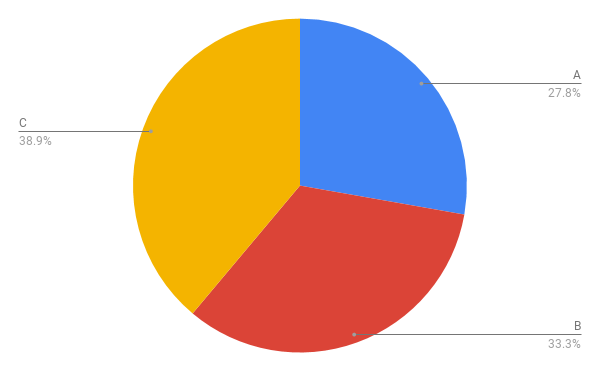
\includegraphics[width=0.5\textwidth]{chart.png}
	\caption{The roulette wheel from my proportional selection example}
	\label{fig:roulette_wheel}
	\end{center}
\end{figure}
Tournament selection could be translated in the following way. Have an empty list which will contain an ordered list of agents. In a loop (until the population is of size 1): select two agents from the population, remove the lowest fitness one and insert it into the list. After the loop insert the last agent into the top of the list. The top of the list always contains the highest fitness agent. Using the same population of agents in the proportional selection algorithm we can give an example of this in table~\ref{tab:tournament_selection}.
\begin{framed}
	\begin{center}
		\begin{tabular}{c|c|c|c}
		Set & Test & Put in List & List\\
		\hline
		${A_1, A_2, B_1, B_2, B_3, B_4, C_1}$ & $(A_1, B_3)$ & $A_1$ & ${A_1}$ \\
		${A_2, B_2, B_3, B_4, C_1}$ & $(B_1, C_1)$ & $B_1$ & ${A_1, B_1}$\\
		${B_2, B_3, B_4, C_1}$ & $(A_2, C_1)$ & $A_2$ & ${A_1, B_1, A_2}$\\
		${B_2, B_3, C_1}$ & $(B_4, C_1)$ & $B_4$ & ${A_1, B_1, A_2, B_4}$\\
		${B_3, C_1}$ & $(B_2, B_3)$ & $B_2$ & ${A_1, B_1, A_2, B_4, B_2}$\\
		${B_3}$ & $(B_3, C_1)$ & $C_1$ & ${A_1, B_1, A_2, B_4, B_2, C_1}$\\
		$\emptyset$	& & $B_3$ & ${A_1, B_1, A_2, B_4, B_2, C_1, B_3}$
		\end{tabular}
		\captionof{table}{The payoff for my indirect reciprocity model}
		\label{tab:tournament_selection}
	\end{center}	
\end{framed}
Fitness proportionate selection seems to translate best to my system as there is an obvious and simple way to select each agents strategy for the new generation using the roulette wheel, unlike the tournament selection process which requires the crossover step. The crossover step requires a chromosome represented as a bit array to produce an offspring from two parents. This is analogous to sexual reproduction, but not the bulding of new agents.\\
Lipowski \textit{et al.}~\cite{lipowski2012roulette} presented an efficient version of roulette wheel selection using stochastic acceptance rather than the searching method used by Francq~\cite{genetic_algorithms}. The stochastic acceptance algorithm works like this: select randomly one of the individuals from the last generations population, with fitness of the individual as $w_i$ and $w_{max}$ the maximal fitness of the generation use the probability $w_i / w_{max}$ to select whether or not to use this agents strategy for a new generation agent, if not repeat. Lipowski \textit{et al.} proved mathematically that the probability distribution of this method and general roulette wheel selection are the same, and that the stochastic acceptance algorithm is more efficient as well.\\
Due to these factors I have decided to use the roulette wheel-selection via stochastic acceptance algorithm proposed by Lipowski \textit{et al.} with a user-selectable chance of random mutation for each new agent.


\subsection{Web Application and Interface}

\section{Development}
Techniques tools and processes?\\
TDD etc.

\section{Testing}
\subsection{Agents Service Testing}
API Testing, Unit Testing.\\

\subsection{Environment Testing}
Unit testing, Integration testing, Regression testing.\\

\subsection{Web App Testing}
\url{https://www.softwaretestinghelp.com/web-application-testing/}

\section{Documentation}

\section{Method}
For discovering evolution of cooperation constraints.

\section{Results}


\chapter{Critical Analysis and Discussion}
Relate to aims.
\section{Analysis}

\section{Discussion}

\section{Conclusions}

%%%% ADD YOUR BIBLIOGRAPHY HERE
\newpage
\bibliography{../../refs.bib}{}
\bibliographystyle{plain}
\addcontentsline{toc}{chapter}{Bibliography}
\footnote{A lot of my background theory work has been completed in my earlier reports so many of the references appear in those reports (see appendix)}
\label{endpage}

\chapter{Professional Issues}
Replacement of people in jobs?\\
AI issues and risks?\\
Relate to project

\chapter{Appendix}
\label{appendix}
Describe the contents of my appendix.

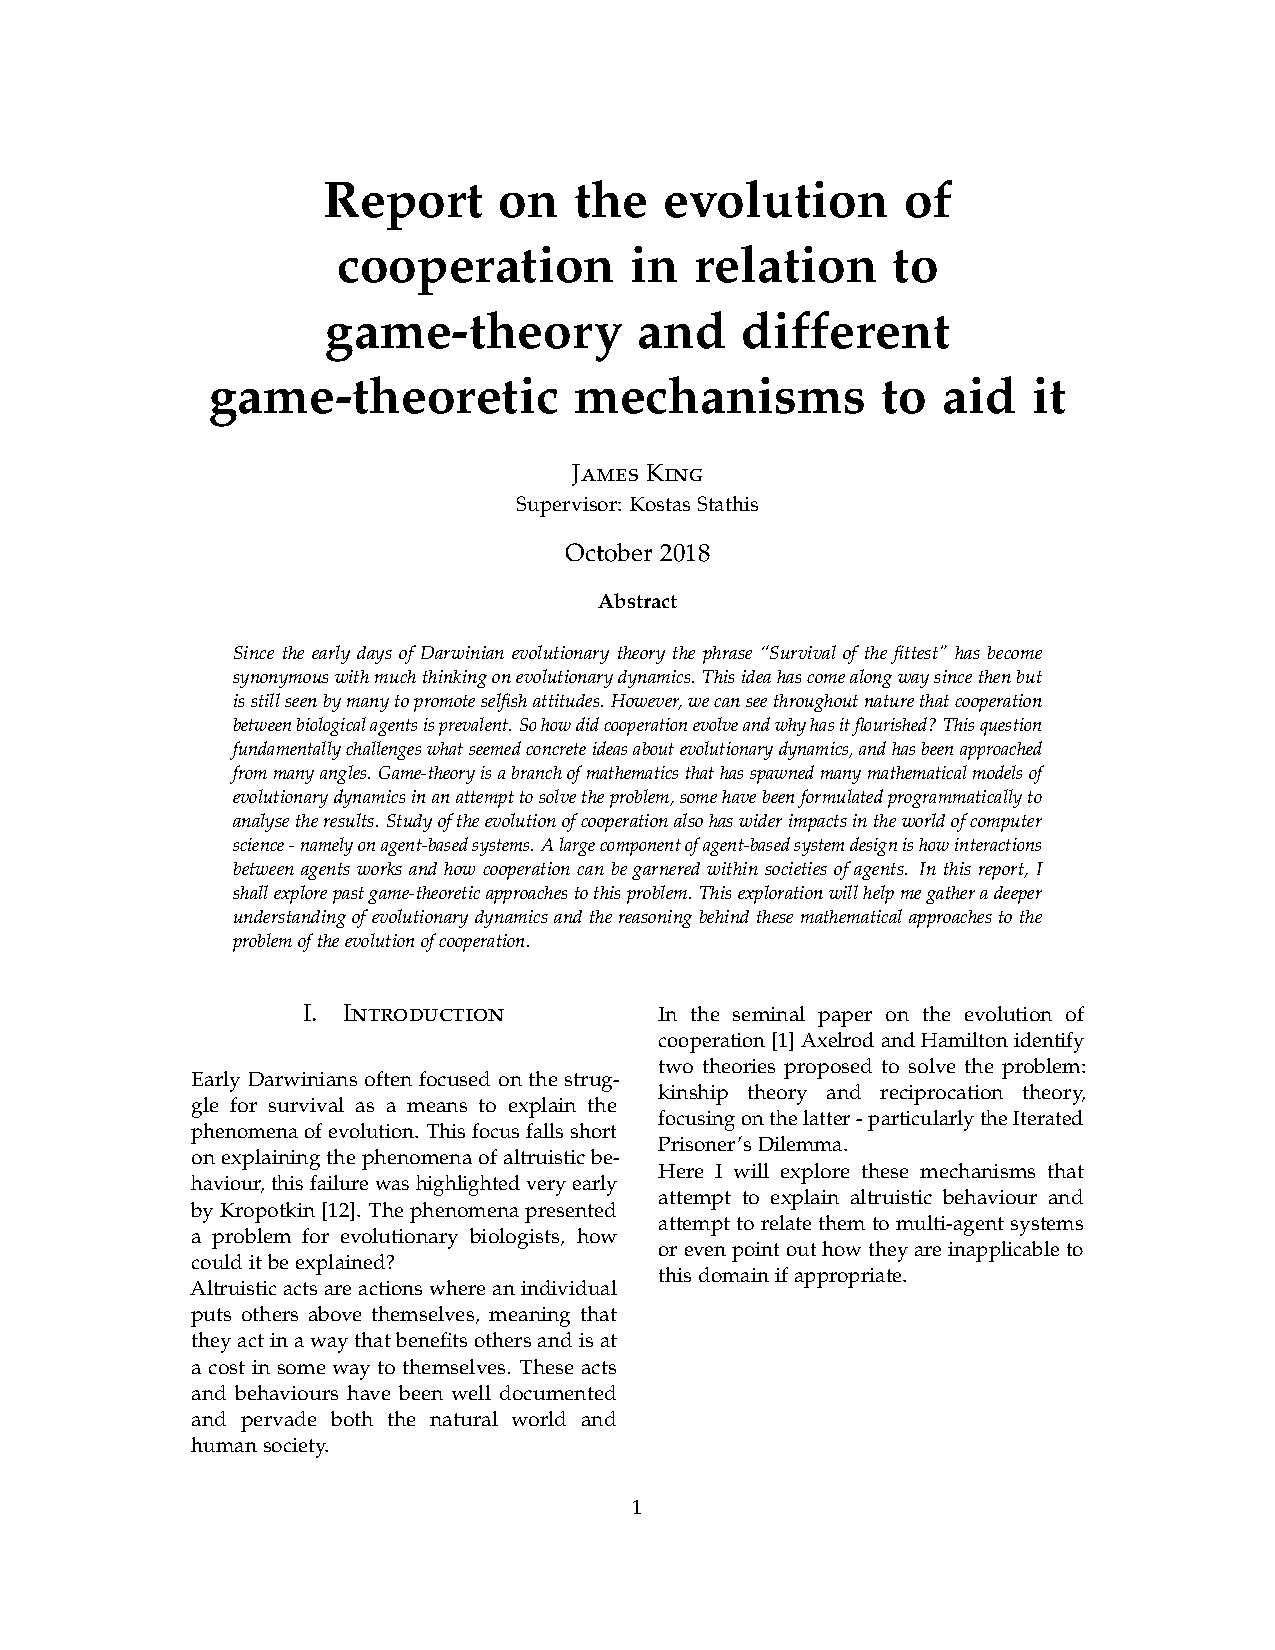
\includepdf[pages=-]{../../EvolCoop/EvolCoopReport.pdf}

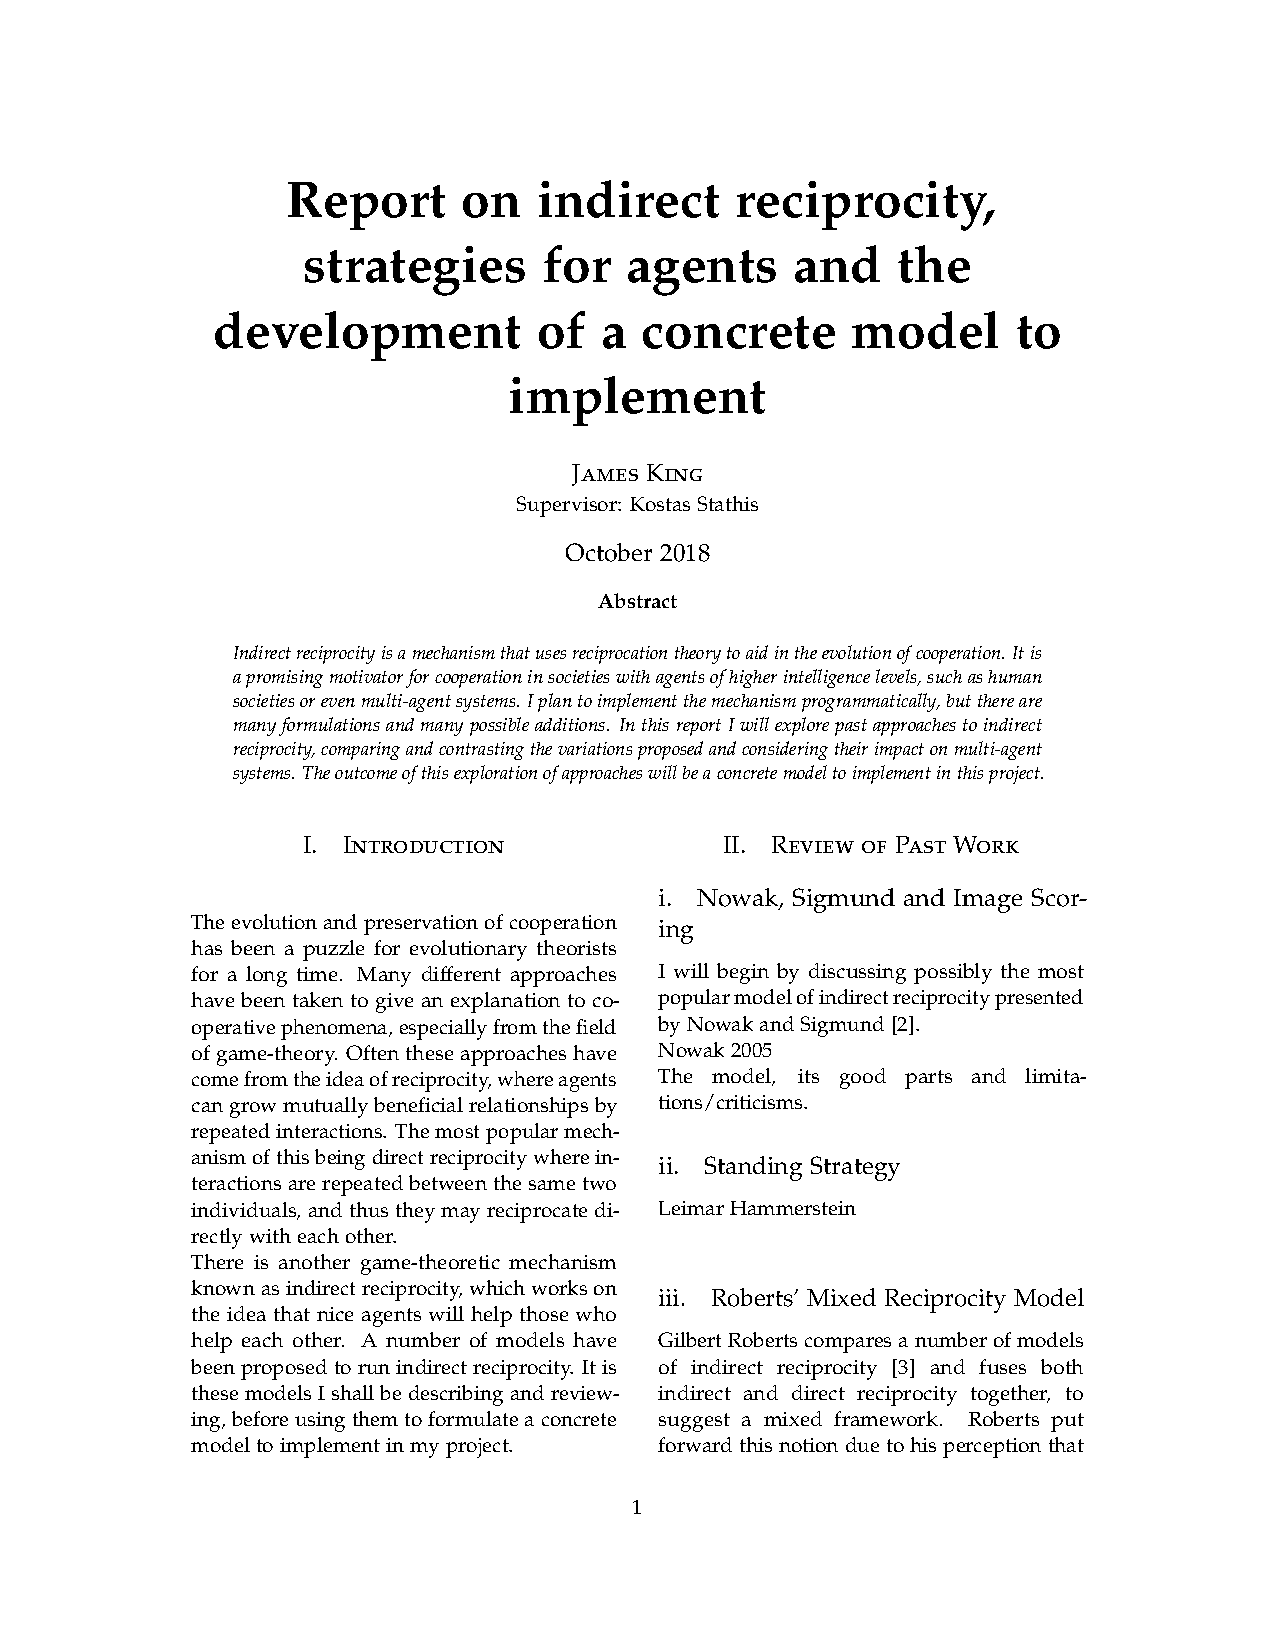
\includepdf[pages=-]{../../IndirRec/IndirRec.pdf}

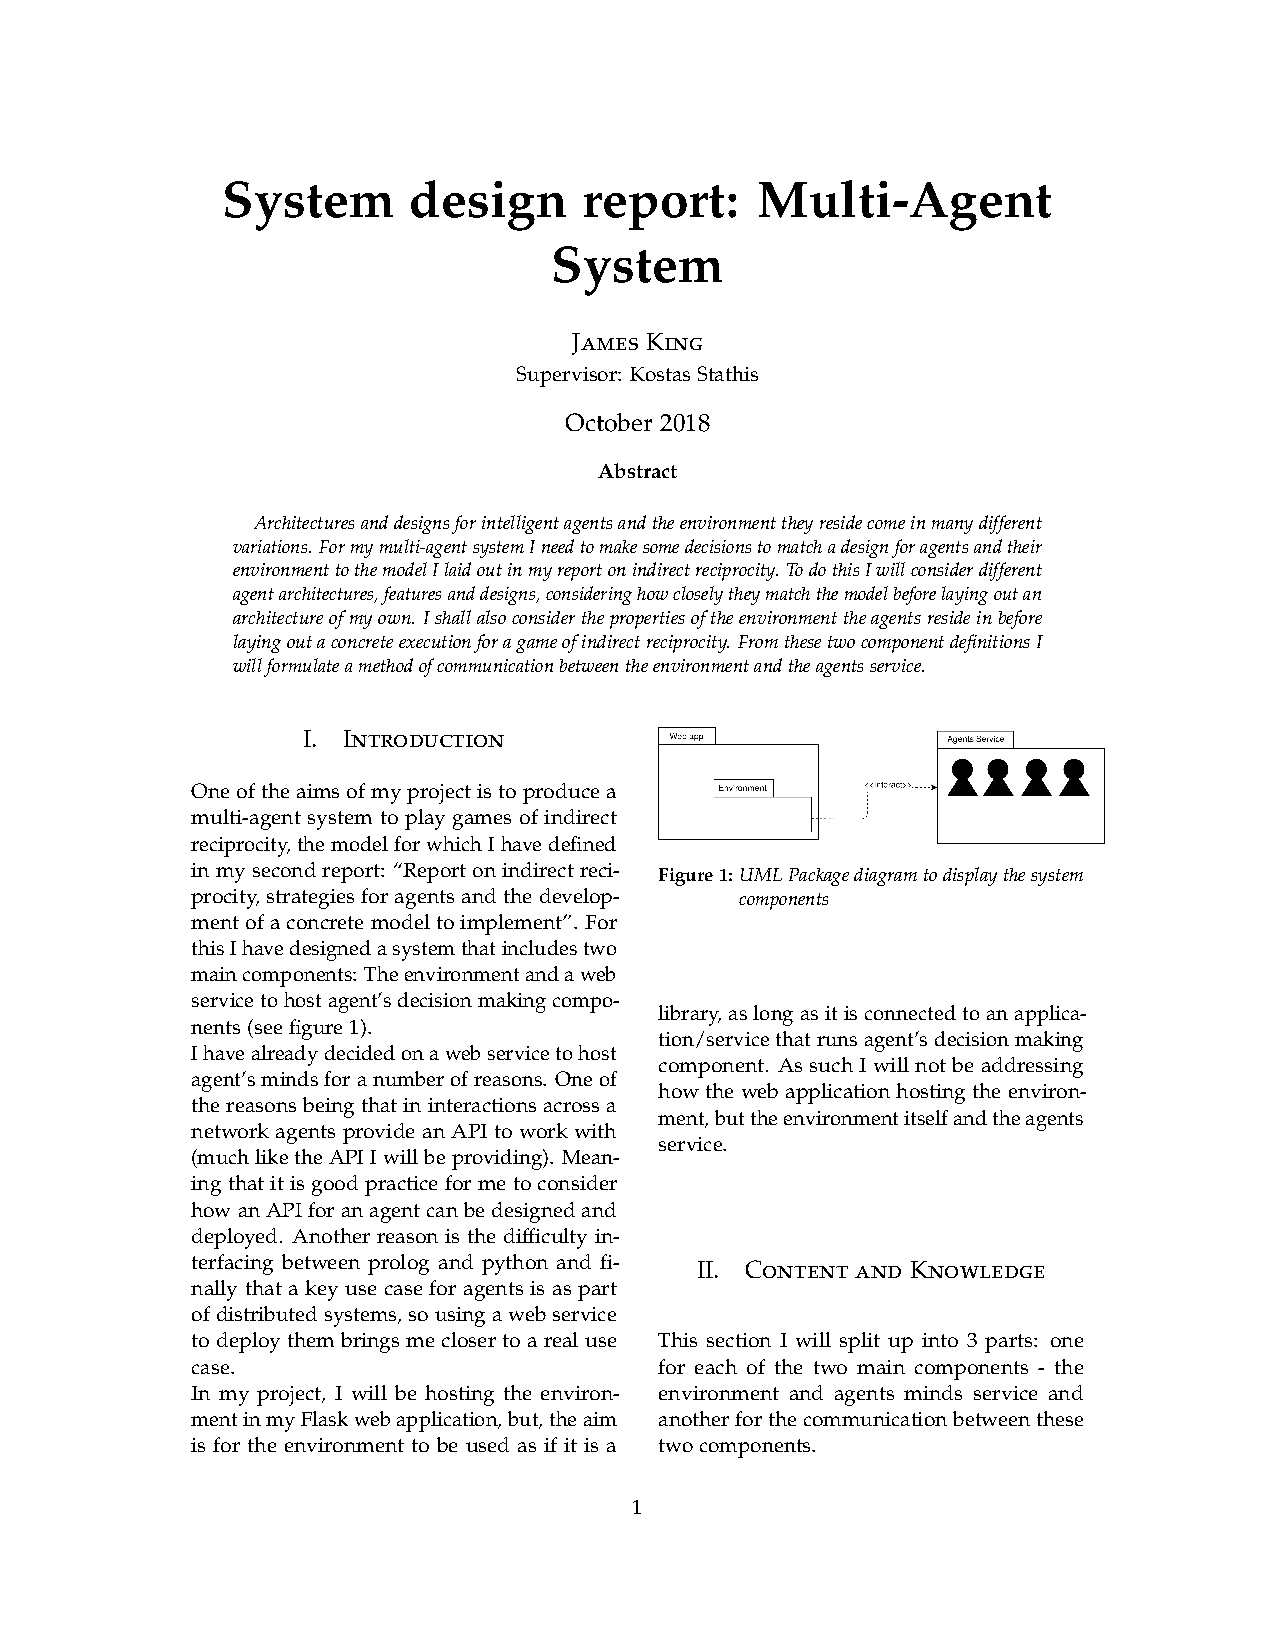
\includepdf[pages=-]{../../SysDesign/SysDesign.pdf}


\end{document}

\end{article}
